% DPF 09 talk on strangeness in nucleon

\documentclass[10pt]{beamer}
\usepackage{amsmath}
\usepackage{mathtools}
%\documentclass[12pt]{beamerthemeSam.sty}
\usepackage{epsf}
%\usepackage{pstricks}
%\usepackage[orientation=portrait,size=A4]{beamerposter}
\geometry{paperwidth=160mm,paperheight=120mm}
%DT favorite definitions
\def\LL{\left\langle}	% left angle bracket
\def\RR{\right\rangle}	% right angle bracket
\def\LP{\left(}		% left parenthesis
\def\RP{\right)}	% right parenthesis
\def\LB{\left\{}	% left curly bracket
\def\RB{\right\}}	% right curly bracket
\def\PAR#1#2{ {{\partial #1}\over{\partial #2}} }
\def\PARTWO#1#2{ {{\partial^2 #1}\over{\partial #2}^2} }
\def\PARTWOMIX#1#2#3{ {{\partial^2 #1}\over{\partial #2 \partial #3}} }

\def\rightpartial{{\overrightarrow\partial}}
\def\leftpartial{{\overleftarrow\partial}}
\def\diffpartial{\buildrel\leftrightarrow\over\partial}

\def\BI{\begin{itemize}}
\def\EI{\end{itemize}}
\def\BE{\begin{displaymath}}
\def\EE{\end{displaymath}}
\def\BEA{\begin{eqnarray*}}
\def\EEA{\end{eqnarray*}}
\def\BNEA{\begin{eqnarray}}
\def\ENEA{\end{eqnarray}}
\def\EL{\nonumber\\}


\newcommand{\map}[1]{\frame{\frametitle{\textbf{Course map}}
\centerline{\includegraphics[height=0.86\paperheight]{../../map/#1.png}}}}
\newcommand{\wmap}[1]{\frame{\frametitle{\textbf{Course map}}
\centerline{\includegraphics[width=0.96\paperwidth]{../../map/#1.png}}}}

\newcommand{\etal}{{\it et al.}}
\newcommand{\gbeta}{6/g^2}
\newcommand{\la}[1]{\label{#1}}
\newcommand{\ie}{{\em i.e.\ }}
\newcommand{\eg}{{\em e.\,g.\ }}
\newcommand{\cf}{cf.\ }
\newcommand{\etc}{etc.\ }
\newcommand{\atantwo}{{\rm atan2}}
\newcommand{\Tr}{{\rm Tr}}
\newcommand{\dt}{\Delta t}
\newcommand{\op}{{\cal O}}
\newcommand{\msbar}{{\overline{\rm MS}}}
\def\chpt{\raise0.4ex\hbox{$\chi$}PT}
\def\schpt{S\raise0.4ex\hbox{$\chi$}PT}
\def\MeV{{\rm Me\!V}}
\def\GeV{{\rm Ge\!V}}

%AB: my color definitions
%\definecolor{mygarnet}{rgb}{0.445,0.184,0.215}
%\definecolor{mygold}{rgb}{0.848,0.848,0.098}
%\definecolor{myg2g}{rgb}{0.647,0.316,0.157}
\definecolor{abtitlecolor}{rgb}{0.0,0.255,0.494}
\definecolor{absecondarycolor}{rgb}{0.0,0.416,0.804}
\definecolor{abprimarycolor}{rgb}{1.0,0.686,0.0}
\definecolor{Red}           {cmyk}{0,1,1,0}
\definecolor{Grey}           {cmyk}{.7,.7,.7,0}
\definecolor{Blue}          {cmyk}{1,1,0,0}
\definecolor{Green}         {cmyk}{1,0,1,0}
\definecolor{Brown}         {cmyk}{0,0.81,1,0.60}
\definecolor{Black}         {cmyk}{0,0,0,1}

\usetheme{Madrid}


%AB: redefinition of beamer colors
%\setbeamercolor{palette tertiary}{fg=white,bg=mygarnet}
%\setbeamercolor{palette secondary}{fg=white,bg=myg2g}
%\setbeamercolor{palette primary}{fg=black,bg=mygold}
\setbeamercolor{title}{fg=abtitlecolor}
\setbeamercolor{frametitle}{fg=abtitlecolor}
\setbeamercolor{palette tertiary}{fg=white,bg=abtitlecolor}
\setbeamercolor{palette secondary}{fg=white,bg=absecondarycolor}
\setbeamercolor{palette primary}{fg=black,bg=abprimarycolor}
\setbeamercolor{structure}{fg=abtitlecolor}

\setbeamerfont{section in toc}{series=\bfseries}

%AB: remove navigation icons
\beamertemplatenavigationsymbolsempty
\title[Exam I Review]{
  \textbf {Exam I Review}\\
%\centerline{}
%\centering
%\vspace{-0.0in}
%\includegraphics[width=0.3\textwidth]{propvalues_0093.pdf}
%\vspace{-0.3in}\\
%\label{intrograph}
}

\author[W. Freeman] {Physics 211\\Syracuse University, Physics 211 Spring 2015\\Walter Freeman}

\date{\today}

\begin{document}

\frame{\titlepage}

\frame{\frametitle{\textbf{Announcements}}
\BI
\item{Exam 1 is on Tuesday}
\item{Homework 2 due tomorrow}
\item{My office hours today are 1:30-3:30 (in the Clinic)}
\item{I will be in the Clinic tomorrow from 10 to 3}
\item{No homework due next week}
\item{Sample exam solutions will be posted tomorrow}
\item{Please arrive a few minutes early if possible to the exam}
\item{We are creating the reference sheet today, during the review}
\EI
}

\frame{\frametitle{\textbf{Exam 1}}
 \BI
 \item{The exam covers kinematics in one and two dimensions}
 \item{Kinematics: how are an object's position, velocity, and acceleration related?}
 \item{\color{Red}The exam will be substantially easier than the homework.}
 \item{You may use a scientific (not graphing) calculator on the exam.}
 \item{Bring: your calculator, pencils, and your physics smarts (frog optional)}
 \EI
}

\frame{\frametitle{\textbf{Exam 1, promises}}
  \BI
\item{There will be one problem where you need the quadratic formula}
  \BI
\item{... this means interpreting the two values it spits out}
  \EI
\item{There will be at least one instance where you need to graph position, velocity, and acceleration}
\item{You will {\it not} need to compute derivatives or integrals algebraically}
  \EI
}

\frame{\frametitle{\textbf{Functions describing motion}}
  \BI
\item{We can specify a function's position, velocity, and acceleration as functions of time: $\vec r(t), \vec v(t), \vec a(t)$}
\item{All of these quantities are vectors; often easier to work with their components}
  \BI
\item{Position: $x(t)$, $y(t)$}
\item{Velocity: $v_x(t)$, $v_y(t)$}
\item{Acceleration: $a_x(t)$, $a_y(t)$}
  \EI
  
\bigskip
\bigskip

\item{If you don't know where to start a problem, figure out $x(t)$, $y(t)$, $v_x(t)$, $v_y(t)$, leaving unknown
  quantities as variables for the time being}
  \EI
}


  \frame{\frametitle{\textbf{Position, velocity, and acceleration}}
    \begin{columns}
      \column{0.125\textwidth}
      \centerline{\Large Position}
      \column{0.2\textwidth}
      \small
      {\color{Red}
        \centerline{(derivative of)}
        \centerline{rate of change of}
      \centerline{$\xleftarrow{\makebox[\textwidth]{}}$}}
      {\color{Green}
      \color{Green}\centerline{$\xrightarrow{\makebox[\textwidth]{}}$}}
      \color{Green}\centerline{area under the curve of}
      \color{Green}\centerline{(integral of)}
      \column{0.125\textwidth}
      \centerline{\Large Velocity}
      \pause
      \column{0.2\textwidth}
      \small
      {\color{Red}
        \centerline{(derivative of)}
        \centerline{rate of change of}
      \centerline{$\xleftarrow{\makebox[\textwidth]{}}$}}
      {\color{Green}
      \color{Green}\centerline{$\xrightarrow{\makebox[\textwidth]{}}$}}
      \color{Green}\centerline{area under the curve of}
      \color{Green}\centerline{(integral of)}
      \column{0.15\textwidth}
      \centerline{\Large Acceleration}
    \end{columns}
  }

  \frame{\frametitle{\textbf{Constant acceleration kinematics}}
    Particularly interesting situation: 
    \BI
  \item{Free fall (as you saw)}
  \item{Any time the force is constant: $F = ma \rightarrow a = F/m$...}
    \EI
    \bigskip
    \pause
    Plan of attack:
    \BI
  \item{We know what the acceleration curve looks like (it's just flat)}
  \item{Figure out the area under the acceleration curve to get the velocity curve}
  \item{Figure out the area under the velocity curve to get the position curve}
    \EI
    \pause
    \bigskip
    \bigskip
    \bigskip
    \bigskip
    Remember the area under the curve of (velocity, acceleration) just gives the {\it change in} (position, velocity) -- \ie initial minus final.

  }


  \frame{\frametitle{\textbf{Constant acceleration kinematics}}
    \centerline{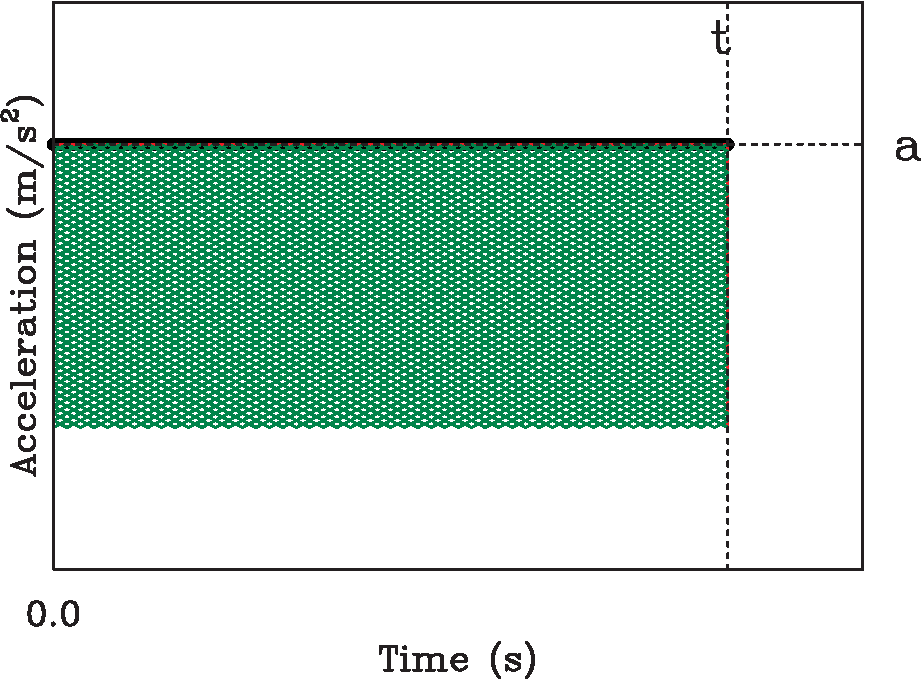
\includegraphics[width=0.6\textwidth]{area-under-a-crop.pdf}}

    \bigskip
    \bigskip

   The area under the curve out to time $t$ is $at$, which gives the change in the velocity.

    \bigskip
    \bigskip

    \centerline{\Large $v(t) - v_0 = at$, so {\color{Red}$v(t) = at + v_0$}}
  }



  \frame{\frametitle{\textbf{Constant acceleration kinematics}}
    \centerline{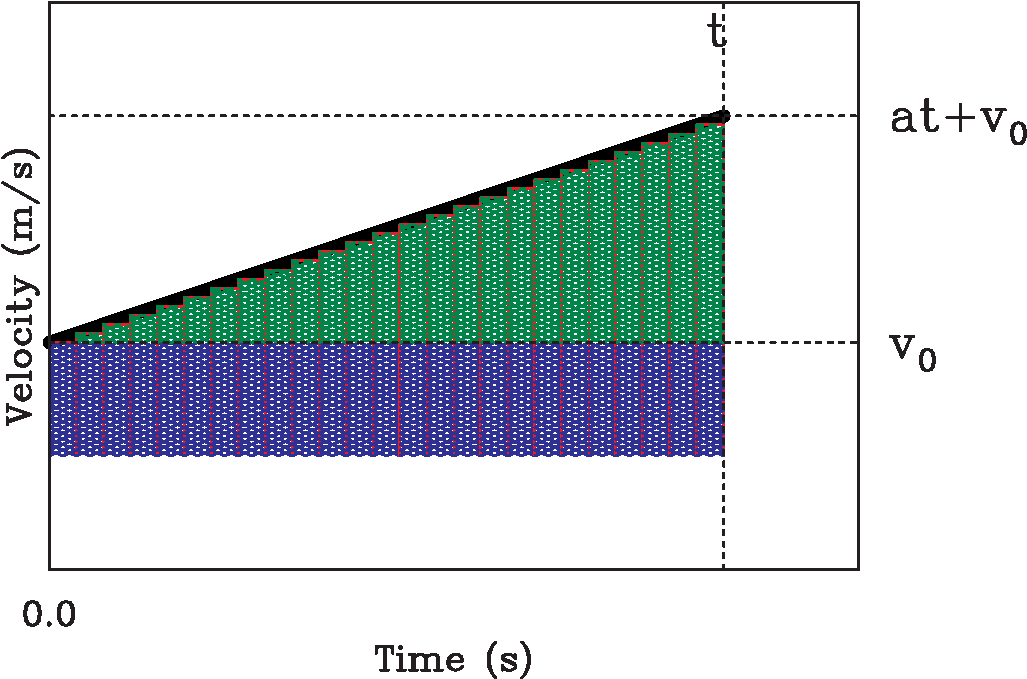
\includegraphics[width=0.6\textwidth]{area-under-v-full-crop.pdf}}

    \bigskip

    Area under blue part: $v_0 t$\\
    Area under green part: $\frac{1}{2} at^2$\\
    Total change in position: $x(t) - x_0 = \frac{1}{2}at^2 + v_0 t$

    \bigskip
    \bigskip
    \centerline{\Large Thus, {\color{Red}$x(t) = \frac{1}{2}at^2 + v_0 t + s_0$}}
  }

  \frame{\frametitle{\textbf{1D Kinematics summary:}}
    
      
    \Large
  Constant acceleration kinematics:
    \begin{align*}
      v(t) &=& at + v_0 \\
      x(t) &=& \frac{1}{2}at^2 + v_0 t + x_0
  \end{align*}

  You can solve one of these for time and substitute into the other to get a third, useful equation:

  $$  v(t) - v_0 = 2a\left[x(t)-x_0\right]  $$

  This is useful when you {\it don't know} and {\it don't care} about the time some motion took.
}

    \frame{\frametitle{\textbf{Vectors: Two ways to describe a vector}}
      \begin{columns}
        \column{0.5\textwidth}
        \centerline{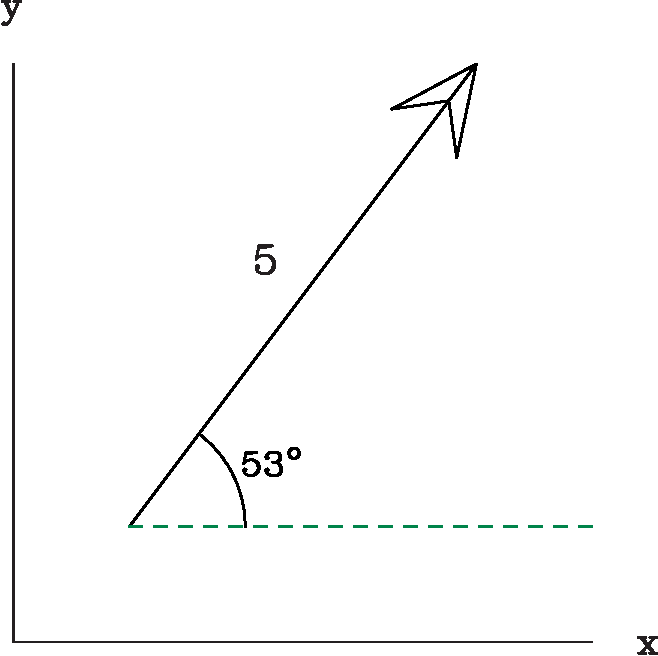
\includegraphics[width=0.7\textwidth]{vector-angle-crop.pdf}}
        \Large
        \centerline{Angle and direction}
        \column{0.5\textwidth}
        \centerline{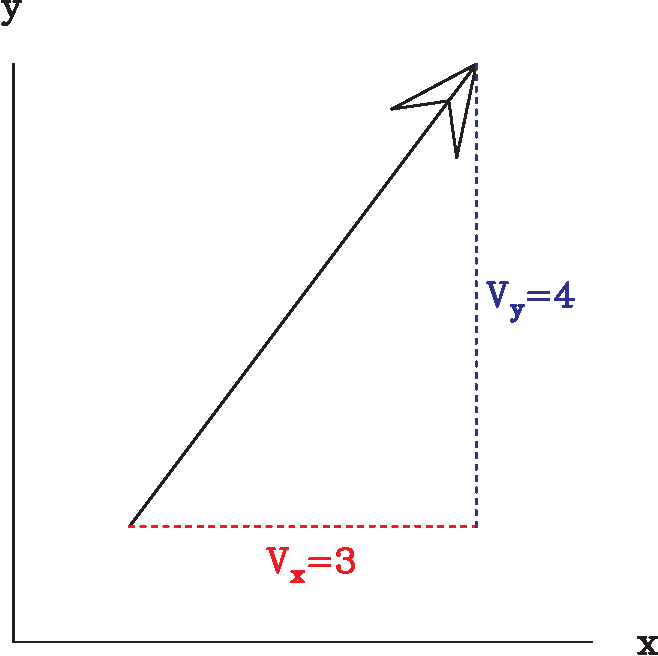
\includegraphics[width=0.7\textwidth]{vector-components-crop.pdf}}
        \Large
        \centerline{X and Y components}
      \end{columns}
      \bigskip
      \bigskip
    }

  
  
  \frame{\frametitle{\textbf{Adding vectors}}
    \centerline{We can also add vectors together by drawing them ``head to tail''. Here are two vectors:}

    \bigskip
    \bigskip

    \begin{columns}
      \column{0.5\textwidth}
      \centerline{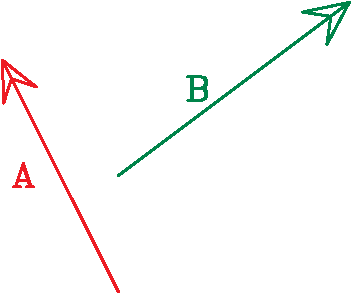
\includegraphics[width=0.6\textwidth]{vshow-crop.pdf}}
      \column{0.5\textwidth}
      \centerline{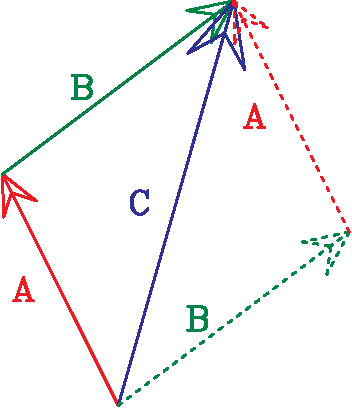
\includegraphics[width=0.6\textwidth]{vadd-crop.pdf}}
    \end{columns}

    \bigskip
    \bigskip

    \Large \centerline{$\color{Red}\vec A + \color{Green} \vec B = \color{Blue} \vec C$}

  }

  \frame{\frametitle{\textbf{Adding vectors: components}}
    \centerline{\Large The component representation is much easier to work with!}

    \Huge\centerline{$\color{Red}\vec A + \color{Green} \vec B = \color{Blue} \vec C \color{Black} \rightarrow {\color{Red} A_x + \color{Green} B_x = \color{Blue} C_x \choose \color{Red} A_y + \color{Green} B_y = \color{Blue} C_y}$}
  }

  \frame{\frametitle{\textbf{Adding vectors: components}}
    \centerline{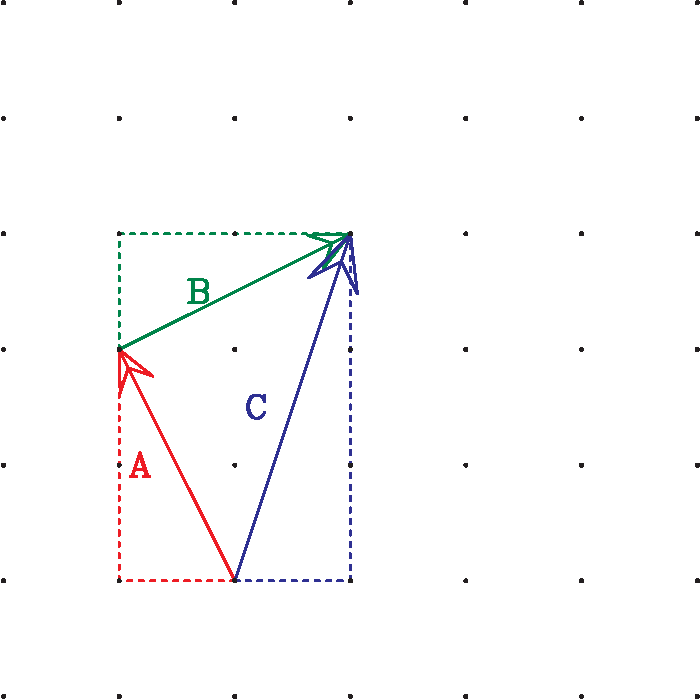
\includegraphics[width=0.4\textwidth]{vaddc-crop.pdf}}

    \large
    \bigskip

    \centerline{To add two vectors, just add their components!}

    \bigskip

    \centerline{This is why it is almost always easiest to work in the component representation!}
  }



  \frame{\frametitle{\textbf{From ``direction and magnitude'' to components}}
    \centerline{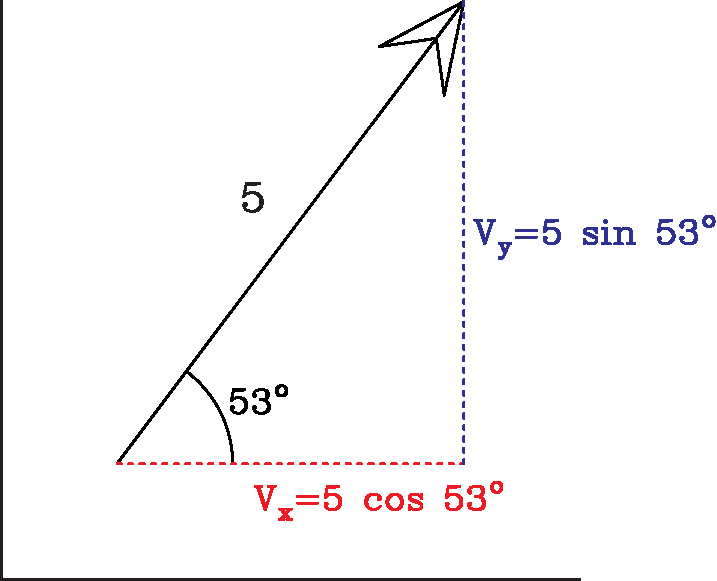
\includegraphics[width=0.6\textwidth]{vector-ang2comp-crop.pdf}}
  }
  
  \frame{\frametitle{\textbf{From components to direction and magnitude}}
    \centerline{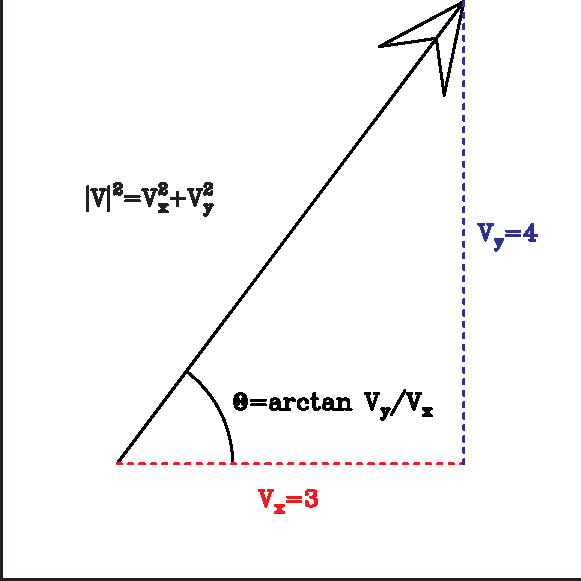
\includegraphics[width=0.6\textwidth]{vector-comp2ang-crop.pdf}}
  }

  \frame{\frametitle{\textbf{Problem solving guide: 1D kinematics}}
    
\BI
\item{Draw a picture!}
\item{Figure out $x(t)$, $v(t)$, $a(t)$ (constant acceleration kinematics}
  \BI
\item{If you have other unknowns that appear in these expressions, that's okay!}
  \EI
\item{Translate physical statements about moments of interest into mathematics}
  \BI
\item{``When does the object hit the ground?'' $\rightarrow$ ``At what time does $y=0$ (or whatever height the ground is)''}
\item{``How high does the object go?'' $\rightarrow$ ``What is the maximum height?'' $\rightarrow$ ``What is $y$
  at the time when $v_y=0$''}
\item{``When do two objects meet?'' $\rightarrow$ ``At what time is $x_1(t) = x_2(t)$''?}
  \EI
\item{Do algebra, solving for the things you want to know}
\item{Make numerical substitutions as the very last step if possible}
\EI
}

  \frame{\frametitle{\textbf{2D kinematics}}
    \Large

    In two dimensions you simply have two copies of all the kinematic relations, one for each:

    \begin{align*}
      v_x(t) =&\, a_x t + v_{x,0} \\
      v_y(t) =& a_y t + v_{y,0} \\
    \end{align*}
    \pause
    \begin{align*}
       x(t) =&\,  \frac{1}{2}  a_x t^2 + v_{x,0} t + x_0\\
      \bigskip
       y(t) =&\, \frac{1}{2}  a_y t^2 + v_{y,0} t + y_0
    \end{align*}
  }

  \frame{\frametitle{\textbf{Problem solving guide: 1D kinematics}}
      \BI
    \item{Draw a picture!}
  \item{Figure out $x(t)$ and $y(t)$, $v_x(t)$ and $v_y(t)$,(constant acceleration kinematics)}
  \item{Remember motion in $x$ and $y$ is separate and independent}
    \item{Translate physical statements about moments of interest into mathematics}
      \BI
    \item{``Where does the object hit the ground?'' $\rightarrow$ ``What is $x$ at the time that $y=0$ (or whatever height the ground is)''}
    \item{``What speed does the object hit the ground with?'' $\rightarrow$ ``What is $|v|=\sqrt{v_x^2 + v_y^2}$ at the time that $y=0$?''}
      \EI
    \item{Do algebra, solving for the things you want to know, going back and forth between representations of vectors ($v_{0,x}$ vs. $v_0 \cos \theta$) as needed}
    \item{Make numerical substitutions as the very last step if possible}
      \EI
    }




  

   \frame{\frametitle{\textbf{Working with variables}}
    \Large 
  \centerline{If you don't know the numerical value of a quantity yet, }
      \centerline{it's fine to leave it as a variable!}

    \bigskip

    \centerline{This is essential for solving many problems.}



\bigskip
\bigskip

\centerline{Example from cannon problem:}

\begin{align*}
  x(t) =& {\color{Red}v_{x,0}} t \\
    y(t) =& -\frac{1}{2} g t^2 + {\color{Red}v_{y,0}} t 
  \end{align*}


}




   \frame{\frametitle{\textbf{Working with variables}}
    \Large 
  \centerline{If you don't know the numerical value of a quantity yet, }
      \centerline{it's fine to leave it as a variable!}

    \bigskip

    \centerline{This is essential for solving many problems.}



\bigskip
\bigskip

\centerline{Example from cannon problem:}

\begin{align*}
  x(t) =& {\color{Red}v_0 \cos 45^o} t \\
  y(t) =& -\frac{1}{2} g t^2 + {\color{Red}v_0 \sin 45^o} t \\
\end{align*}

  \centerline{(I leave the rest to you for now...)}

}

      \frame{\frametitle{\textbf{The roadrunner problem}}
\large
The position of the car is given by the ordinary 1D kinematics relation:

\bigskip

$x(t) = \frac{1}{2} at^2 + v_0 t = \frac{1}{2} (-9) t^2 + (30.6) t$ (mks units)

\pause
\bigskip

We care about the time when it meets up with the position of the roadrunner, which is 30m. So we set $x(t) = 30$ and solve.

\centerline{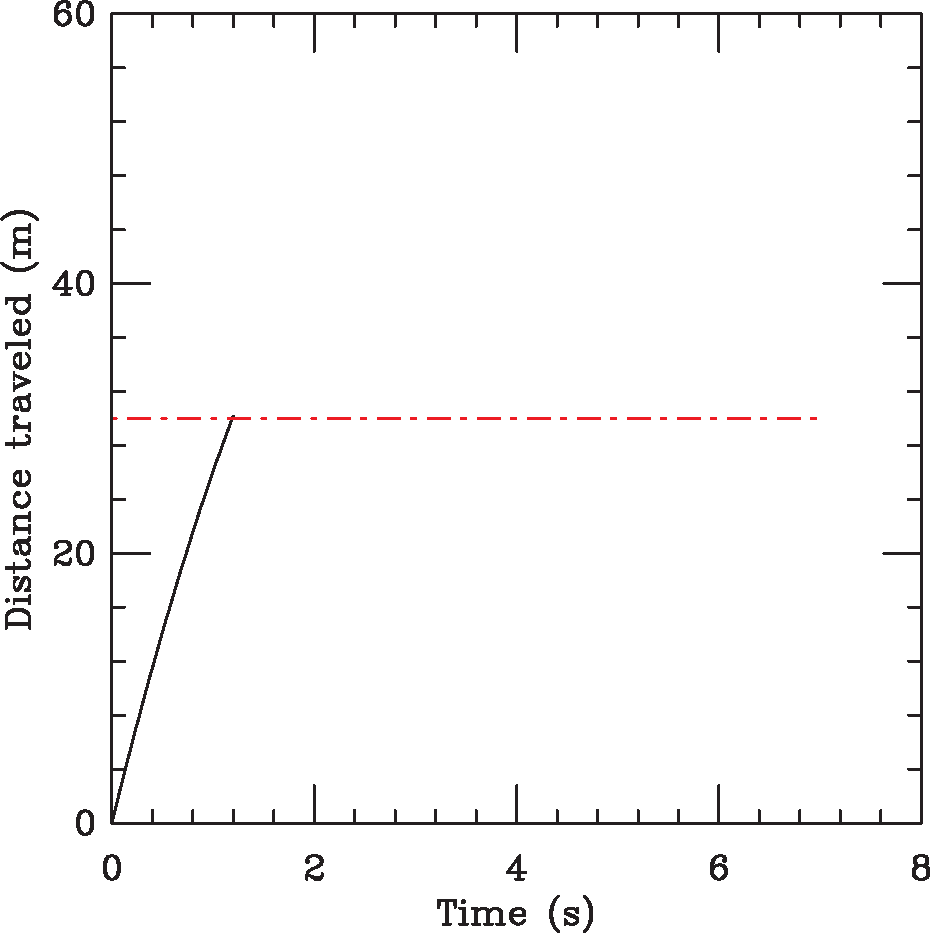
\includegraphics[width=0.3\textwidth]{rr1-crop.pdf}}

This seems easy enough, but the quadratic formula gives us two solutions! What happened?

}

\frame{\frametitle{\textbf{The roadrunner problem}}
\large
The position of the car is given by the ordinary 1D kinematics relation:

\bigskip

$x(t) = \frac{1}{2} at^2 + v_0 t = \frac{1}{2} (-9 m/s^2) t^2 + (30.6 m/s) t$

\bigskip

We care about the time when it meets up with the position of the roadrunner, which is 30m. So we set $x(t) = 30$ and solve.

\centerline{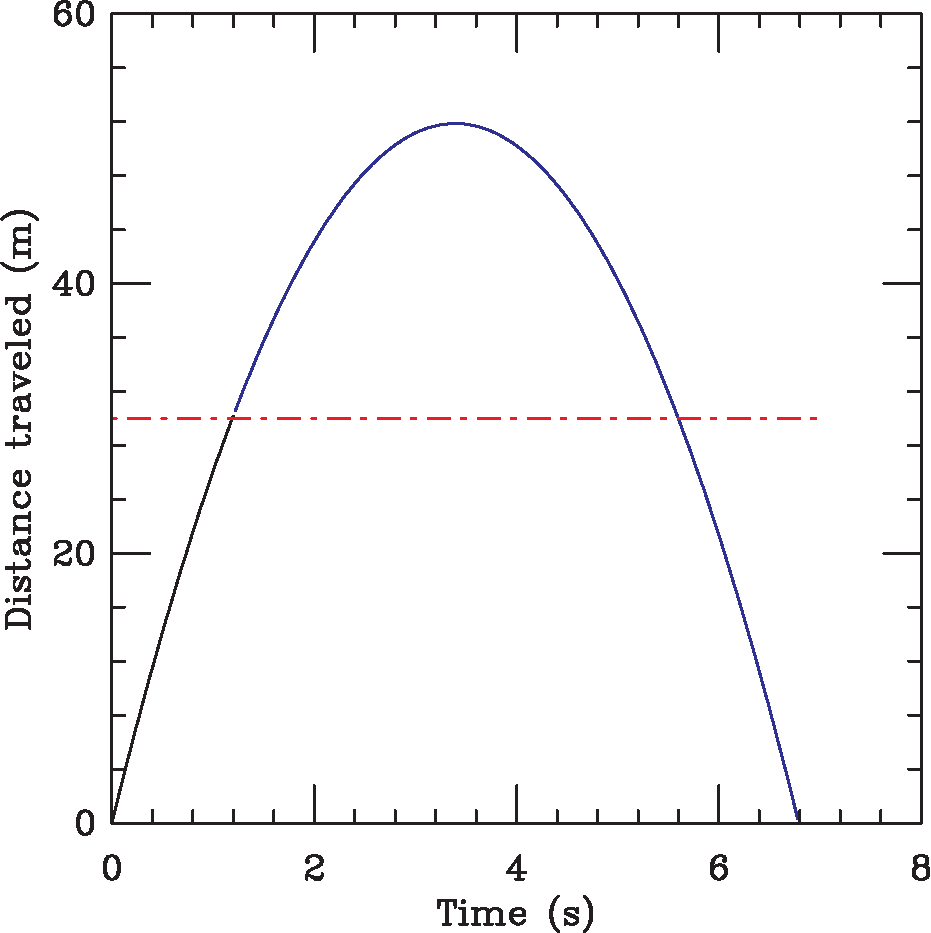
\includegraphics[width=0.3\textwidth]{rr2-crop.pdf}}

\pause

Moral of the story: mathematics is a very blunt tool!

}


\frame{\frametitle{\textbf{Throwing a stone onto a slope}}
  A hiker kicks a stone off of a mountain slope with an initial velocity of 3 m/s horizontally. If the mountain has a slope
  of 45 degrees, how far down the slope does it land?

  \pause
\BI
\item{  Same kinematic relations as before (this is always a good starting point!)}


 $x(t) = {\color{Red} \frac{1}{2} a_xt^2} + v_{0,x} t + \color{Red}x_0$
  
 $y(t) = {\frac{1}{2} a_yt^2} + {\color{Red}v_{0,y}} t + y_0$

\bigskip
\pause

\item{Now the condition for ``rock hits ground'' requires some thought:}
\pause
\item{The rock hits the ground when $x(t)=-y(t)$}

  
  $v_{0,x}t=\frac{1}{2}gt^2 \rightarrow t=\frac{2v_{0,x}}{g}$

  \pause
\item{This gives us $x(t) = \frac{2v_{0,x}^2}{g}$}
\item{$y(t)$ will have the same magnitude: the Pythagorean theorem gives $|r| = 2 \sqrt{2} \frac{v_{0,x}^2}{g}$}
\EI
}

  
\frame{\frametitle{\textbf{A rocket}}
 \Large
  A rocket is launched from rest on level ground. While its motor burns, it accelerates at 10 m/s at an angle 30 degrees
  below the vertical. After ten seconds its motor burns out and it follows a ballistic trajectory until it hits the ground.

  \bigskip

  How far does it go?

}


      \end{document}
